\section{VISIÓN COMPUTACIONAL}
    
    \subsection{PROCESAMIENTO DE IMÁGENES}
        Es la aplicación de operaciones del procesamiento de señales unidimensionales sobre imágenes, interpretadas como una señal bidimensional.
        \subsubsection{REPRESENTACIÓN DE IMÁGENES EN UNA COMPUTADORA}
        Una imágen $I$ está compuesta por píxeles $(x, y, v)$ cuyos componentes son una coordenada $(x, y) \in \mathbb{Z}^2$ y un valor $v \in \mathbb{Z}^c$, con $c$ el número de canales de color, siendo $c=1$ una imágen a escala de gristes y $c=3$ una imágen a colores Rojo, Verde y Azúl (RGB por sus siglas en inglés), definida sobre un conjunto $\Omega$. 
        
        \begin{equation}
            \Omega = \{(x, y)| 1 \leq x \leq N_{columnas} \land 1 \leq y \leq N_{filas}\} \subset \mathbb{Z}^2
        \end{equation}
        
        la representación que vemos en la computadora se le llama modelo grid cell, donde cada píxel es un cuadrado pequeño o celda con una intensidad de grises o canales RGB \citep{10.5555/2584519} con valores $0 \leq I_{x, y} \leq 255$.

        \begin{figure}[H]
            \centering
            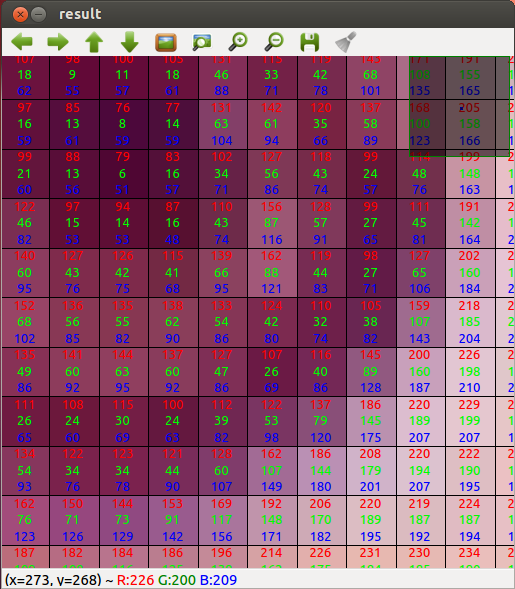
\includegraphics[scale=0.25]{imagenes/pixels}
            \caption{Intensidad de los canales de color RGB\\ Fuente: \citep{montabone_2012}}
        \end{figure}
        % \vspace{-8mm}
        % \begin{center}
        %     Fuente: \citep{montabone_2012}
        % \end{center}
        % \subsubsection{TRANSFORMACIONES DE PERSPECTIVA}
        % Page 359 birds eye
        % \subsubsection{DETECCIÓN DE BORDES}
        \subsubsection{CONVOLUCIÓN}
        Cuando deseamos aplicar alguna transformación de alguna imagen $I$ a alguna imagen $I'$ como difuminados, realce de bordes o extracción de alguna característica, debemos aplicar un operador local lineal entre un filtro que acentúe la característica en la imagen $I$.
        
        El filtro denotado por $W$ es una matriz cuadrada de dimensión $(2k+1) \times (2k+1)$, aplicada en forma de ventana deslizante sobre cada pedazo de la misma dimensión de la imagen original, siendo $(x, y)$ el punto central de cada sección sobre la que se opera, se define la convolución como:
        
        \begin{equation}
            I'_{x,y} = \frac{1}{s} \sum_{i=-k}^{k} \sum_{j=-k}^{k} w_{i, j}\cdot I_{x+i, y+j}
        \end{equation}
        
        y se denota por el operador $*$ como $I' = I*W$ con $s$ un valor de escala \citep{10.5555/2584519}. Esta operación es equivalente a si aplastamos el filtro y la sección de la imagen en dos vectores, y realizamos una combinación lineal o suma ponderada de sus valores.
        \subsubsection{DIFUMINADO}
        Para aplicar un difuminado o blur a una imagen se aplica comúnmente un filtro normal o gaussiano, para esto se define que el filtro se distribuye normal bivariante:
        
        \begin{equation}
            W \sim \mathcal{N}\left(\mu=\begin{bmatrix}
                                    0\\
                                    0
                                    \end{bmatrix},
                                    \Sigma=
                                    \begin{bmatrix}
                                    \sigma^2 & 0\\
                                    0 & \sigma^2
                                    \end{bmatrix}\right)
        \end{equation}
        
        Si generamos un filtro o kernel como una muestra de la distribución normal, de tamaño $6\sigma-1$ redondeado al entero impar más cercano, por la regla empírica de las tres desviaciones estándar, y escalado por $\frac{1}{s}$, obtenemos el un filtro que ponderará más los píxeles cercanos al centro, de manera que el difuminado mantendrá las características de cada sección de la imagen.
        
        \begin{figure}[H]
            \centering
            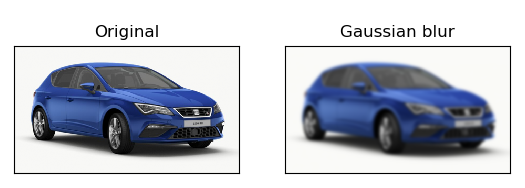
\includegraphics[scale=0.48]{imagenes/blur}
            \caption{aplicación del filtro gaussiano\\ Fuente: Elaboración propia}
        \end{figure}
        % {\centering Fuente: Elaboración propia\par}
        \subsubsection{DETECCIÓN DE BORDES}
        Un borde es esencialmente un cambio brusco de intensidad de los valores de los píxeles en una sección de una imagen, de esta manera, para detectar bordes debemos aplicar algún tipo de suma ponderada que dé como resultado un valor alto si existe un cambio brusco de intensidad, y un valor bajo en caso contrario. 
        Es bajo esta premisa que se propone el filtro Sobel \citep{sobel}, usado luego de aplicar un difuminado gaussiano, y consiste en una combinación entre una convolución gaussiana
        $$\mathcal{G} = \begin{bmatrix}
                                    1\\
                                    2\\
                                    1
                        \end{bmatrix}$$
        \noindent y una aproximación de la derivada parcial de la imagen en espacio discreto con $\Delta_x = \Delta_y = 1$ en cada dimensión
        
        $$\frac{\partial I_{x, y}}{\partial x} = \frac{I_{x+\Delta_x, y} - I_{x-\Delta_x, y}}{\Delta_x}$$
        
        $$\frac{\partial I_{x, y}}{\partial y} = \frac{I_{x, y+\Delta_y} - I_{x, y-\Delta_y}}{\Delta_y}$$
        
        \noindent dando como filtro unidimensional
        
        $$\mathcal{D} = \begin{bmatrix}
                                    1 & 0 & -1
                        \end{bmatrix}$$
                        
        \noindent combinando ambos filtros unidimensionales obtenemos el filtro Sobel para cada dimensión
        \begin{equation}
        \begin{aligned}
        S_x &=  \begin{bmatrix}
                 1\\
                 2\\
                 1
                 \end{bmatrix}
                 \begin{bmatrix}
                 1 & 0 & -1
                 \end{bmatrix}=
                 \begin{bmatrix}
                 1 &  0 &  -1\\
                 2 &  0 &  -2\\
                 1 &  0 &  -1\\
                 \end{bmatrix}\\
        S_y &=  \begin{bmatrix}
                 1\\
                 0\\
                 -1
                 \end{bmatrix}
                 \begin{bmatrix}
                 1 & 2 & 1
                 \end{bmatrix}=
                 \begin{bmatrix}
                 1 &  2 &  1\\
                 0 &  0 &  0\\
                 -1 &  -2 &  -1\\
                 \end{bmatrix}
        \end{aligned}
        \end{equation}
        
        \noindent al ser esta la derivada parcial con respecto de cada dirección, podemos calcular la magnitud mediante la norma $L_2$
        
        \begin{equation}
            \nabla I_{x, y} = \sqrt{S_x^2 + S_y^2}
        \end{equation}
        
        \noindent y la dirección del gradiente
        
        \begin{equation}
            \theta = tan^{-1}\left(\frac{S_y}{S_x}\right)
        \end{equation}
        
        \begin{figure}[H]
            \centering
            % 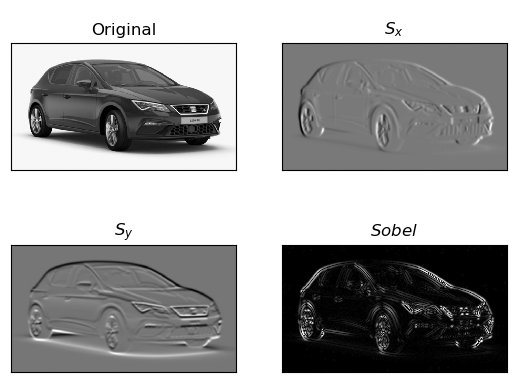
\includegraphics[scale=0.5]{imagenes/sobel_filters}
            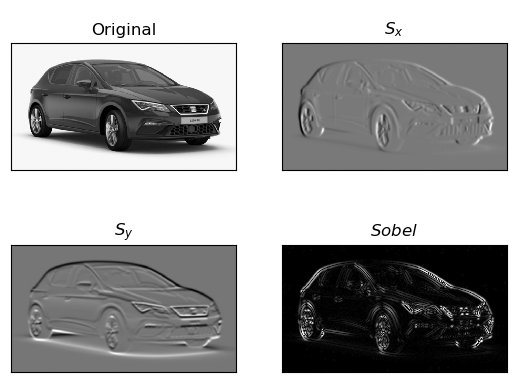
\includegraphics[scale=0.47]{imagenes/sobel_filters}
            \caption{filtro Sobel por dimensiones y total\\ Fuente: Elaboración propia}
        \end{figure}
        % \vspace{-8mm}
        % \begin{center}
        %     Fuente: Elaboración propia
        % \end{center}
        \subsubsection{FILTRO CANNY}
        Los bordes detectados por el filtro Sobel no son independientes de la resolución, por lo que pueden ser más gruesos o delgados dependiendo de la imagen, y detectar como bordes transiciones de iluminación que no lo son necesariamente, es con el fin de refinar este resultado que propone el filtro Canny, que se aplica a la salida de un filtro Sobel \citep{canny}.
        Para aplicar este filtro primero se redondean las direcciones a múltiplos de $45^\circ$ y se procede a verificar si comparado con los píxeles vecinos en esa sección y esa orientación, es el valor máximo o no, en caso que no lo fuese se anula el valor del píxel volviéndolo $0$, caso contrario se continúa con el paso de probar límites de valores, dónde se eligen dos valores $t_{alto}$ y $t_{bajo}$, si un píxel cumple $I_{x,y} \ge t_{alto}$ entonces se considera borde, entonces se verifica cuáles de los 8 píxeles vecinos cumplen $I_{x\pm 1, y \pm 1} \ge t_{bajo}$, finalmente los píxeles que cumplan esta condición se marcan con el máximo valor de un píxel, $255$ y se repite el procedimiento. Si no se cumple la primera condición con el límite alto se asigna el valor $0$ al píxel, obteniendo así una imagen binaria donde los píxeles que representan un borde son de color blanco y los que no, son negros.
        
        \begin{figure}[H]
            \centering
            % 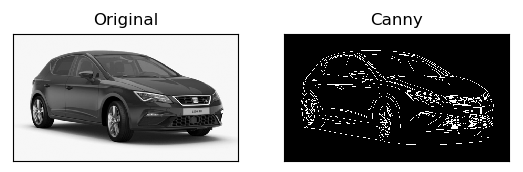
\includegraphics[scale=0.7]{imagenes/canny}
            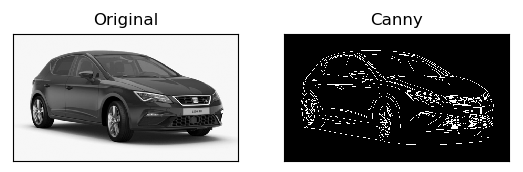
\includegraphics[scale=0.55]{imagenes/canny}
            \caption{aplicación del filtro Canny\\ Fuente: Elaboración propia}
        \end{figure}
        % \vspace{-8mm}
        % \begin{center}
        %     Fuente: Elaboración propia
        % \end{center}
        % \subsubsection{DESCRIPTORES}
        % \subsubsection{CLASIFICACIÓN DE IMÁGENES}
    % \subsection{DETECCIÓN DE OBJETOS}
    % \subsection{SEGMENTACIÓN SEMÁNTICA}
